\section{ Základné pojmy }
V nasledujúcom texte sa budú používať tieto pojmy, ktoré sú zavedené pre potrebu bakalárskej práce a nepoužívajú sa v inom zmysle:
\begin{description}
\item[Mapa (bojisko)]\hfill \\
	Mapou nazveme prostredie, kde sa odohráva boj (testovanie algoritmov )
\item[Objekt]\hfill \\
	Pod objektom rozumieme akýkoľvek prvok na mape, ktorá smie priamo alebo nepriamo ovplyvňovať výsledok vykonávania algoritmov. Tento pojem nemá žiadnu súvislosť s pojmom Objekt, ako je známy z objektových programovacích jazykov.
\item[Algoritmus]\hfill \\
	Algoritmom nazvime postup, zapísaný pomocou nejakého jazyka. 
\item[Robot]\hfill \\
	Pod pojmom robot rozumieme objekt, ktorého chovanie je dané algoritmom.
\item[Misia]\hfill \\
	Misiou nazvime algoritmus robota, ktorý predpokladá splnenie nejakých podmienok. Úspešne ukončenou misiou nazveme algoritmus, o ktorom vieme s naprostou istotou povedať, že tieto podmienky sú splnené.
\item[Súper robota]\hfill \\
	Pod týmto pojmom sa rozumie robot, ktorého algoritmus môže byť potenciálnou hrozbou pre robota.
\item[Spojenec robota] \hfill \\
	Spojencom robota A je taký robot B, o ktorom algoritme robot A predpokladá, že prispeje k úspešnej misii robota A. %?OMG!
\end{description}

\section{ Požiadavky }\label{poziadavky}
	Náplnou bakalárskej práce je vytvoriť čo najuniverzálnejšie prostredie pre skúšanie algoritmov pre umelú inteligenciu. Aplikácia algoritmu, ktorý bol programom bakalárskej práce označený za víťazný, by mal aj v reálnej hre s rovnakými parametrami a cieľami uspieť. Preto  boli  v tejto práci zvolené nasledujúce požiadavky:
\begin {itemize}
\item Hráč si bude moc napísať algoritmus chovania pre jedného alebo viac robotov naraz. Užívateľsky je príjemnejšie mať pokope robotov, ktorí budú spúšťaní vždy spoločne. Výhodou je aj ľahké prípadné rozšírenie o spolupracujúcich robotov, ako je to napríklad v hre Dragon Age.
\item Všetky vstupné algoritmy rôznych robotov by sa mali dať skombinovať.
	\\Týmto spôsobom sa bude dať okamžite spustiť skupina robotov spolu s inou skupinou a nebude treba ich manuálne upravovať pred spustením.
\item Algoritmus sa musí dať napísať v jazyku, ktorý je ľahko pochopiteľný, dostatočne detailný a ľahko rozšíriteľný.
	Rozšírením sa myslí napríklad reakcie robota, alebo zakomponovanie novej činnosti, ktorú môže robot vykonávať
\item Napísaný algoritmus by sa mal dať rozdeliť na malé čati, ktorých vykonávanie bude ľahko sledovateľné.
\item Užívateľ bude môcť vypustiť do mapy jedného alebo viac robotov do dopredu určených miest.
\item Užívateľ bude môcť nastaviť parametre robota, ovplyvňujúce jeho chovanie, a to globálne alebo lokálne. Globálne nastavenie sa prejaví u každého robota. Lokálne nastavenie je vlaste prepísanie čísla v globálnom nastavení, ale pltné len pre jedného robota, ktorého vstup obsahuje prepísanie tejto hodnoty.\\
	V rôznych hrách sa totiž prejavujú rozlične vlastnosti robotov, ako napríklad ničivosť zbraní.
\item Užívateľ by mal mať možnosťa definovať, kedy sa misia úspešne ukončila. \\
	Niektoré hry ako napríklad Thief alebo Capture the flag totiž podmieňujú úspešné ukončenie misie inými podmienkami ako prázdnym bojiskom.\\
	Do úvahy boli zobraté najčastejšie verzie úloh z RPG a bojových hier. To sú napríklad vykonanie akcie v nejakej lokácií, ( akcia sa môže líšiť v každej hre), odmedzenie na počet zabitých nepriateľov, ako je to napríklad v hre Thief, a zameranie sa na určitého neprateľa. Tento cieľ sa vyskytol vo viacerých hrách, ako reprezentanta môžeme uviesť napríklad Baldurs gate.
\item Program by mal rozhodovať, kedy simuláciu ukončiť.\\
	Na úspech misie sa dá alebo nazerať dvoma spôsobmi - pokiaľ sú splnené všetky podmienky zadané užívateľom alebo neexistuje nič, čo by úspech prekazilo. Druhá podmienka je pomerne diskutabilná, pretože v tomto prípade by úspechu mohlo zabrániť samotný algoritmus, ale keďže to inak ako dokončením simulácie nezistíme, je možné bez ujmy na obecnosti predpokladať, že algoritmus raz k splneniu podmienky dojde a vyhlásiť misiu za úspešnú.
\item V každom okamihu sa robot bude vedieť zmysluplne rozhodnúť, ktorú inštrukciu vykonať. Táto požiadavka naráža na základný problém, čo sa má stať v okamihu, keď robot vykoná všetky inštrukcie. 
\end{itemize}

%%%%%%%%%%%%%%%%%%%%%%%%%%%%%%%%%%%%%%%%%%%%%%%%%%%%%%%%%%%%%%%%%%%%%%%%%%%%%%%%%%%%%%%%%%%%%%%%%%%%%skor do analyzy?
%\section { Codewars } %struktura aneb analyza
\subsection {Získavanie dát}
\indent Najskôr bolo nutné rozoznávať vstupné data. Na výber sa ponúka niekoľko možností. Bolo by možné implemetovať priamo do aplikácie editor vstupov. Keďže ale hlavne v unixe, pre ktorý bol program primárne vyvíjaný, majú užívatelia svoj preddefinovaný editor, ktorý ovládajú a kde majú nadefinované makrá a skratky. Vzhľadom na túto okolosť je užívateľsky príjemnejšie neimplementovať nič nové a ponechať užívateľovi jeho preddefinovaný editor.\\
Algoritmy robotov je teda výhodné načítavať zo súboru, kde sú popísané pomocou jazyka. A keďže štardartne bude mať užívateľ tieto vstupy pospolu pre rýchlejší prístup, bez ujmy na obecnosti na neho môže byť kladený nárok na pomenovanie vstupu s preddefinovanou koncovkou a v predefinovanom adresári. V práci sa použila koncovka ''input'' a adresár ''inputs'', ktorý sa pre lepšiu lokalizáciu bude nachádzať v adresári so spustiteľným súborom aplikácie.

\subsection{ Definícia jazyka vstupov }
Jazyk, v ktorom má užívateľ napísať svoj algoritmus, musí byť ľahko pochopiteľný, jednoduchý na porozumenie a hlavne obsahujúci funkcie pre popis virtuálneho sveta. Napríklad funkcie pre získavanie informácií o objektoch, ktoré robot vidí, kde sa nachádzajú, a pod. . Preto musí byť tiež rozšíriteľný na ďalšie udalosti, ktoré by mohli nastať. Na výber sa ponúka niekoľko scriptovacích jazykov, ako napríklad \emph{Lua}, vytvorenie vlastného jazyka pomocou parsovacích nástrojov, ako je napríklad \emph{Bison} a \emph{Flex}, alebo ponechanie napísania vstupu v jazyku aplikácie.Všetky prístupy majú svoj výhody aj nevýhody.
\begin{description}
	\item[Objektový jazyk aplikácie]\hfill \\ Výhodou tohoto prístupu je, že nie je potrebné nič naimplementovať, stačí definovať rozhranie, aké musí súbor mať, poprípade knižnice, hlavičky/package, v závislosti na zvolenom jazyku. Nevýhodou tohoto prístupu je nutnosť kompilovať, čo môže nepríliš oboznámených užívateľov k smrti vydesiť. Ďalšou malou nevýhodou je nutnosť poznať daný jazyk minimálne na základnej úrovni a tiež nutnosť poznať implementačné detaily.Rovnako by bolo pomerne obtiažne určiť, kde presne sa aktuálne nachádza kód robota a ktorú metódu/funkciu bude vykonávať následovne. Tiež sa nedá kontrolovať vyťaženosť pamäte.
	\item[Scriptovací jazyk]\hfill \\ Jedná sa napríklad o scriptovací jazyk \emph{Lua}, ktorú už bol úspešne použitý napríklad pri hre Baldurs Gate na prispôsobenie vzhľadu sveta. Výhodou tohoto jazyka je pomerne prehľadná kompilácia, multiplatformnosť, prehľadné písanie kódu a kompilácia za behu programu. Malou nevýhodou je nutnosť inštalovania Lua virtua machine, ktorá, podobne ako Java Virtual Machine, je virtuálny stroj určený pre vykonávanie inštrukcií Lua scriptu
	\item[Parsovacie nástroje]\hfill \\ Jedná sa napríklad o nástroje Bison a Flex. Výhodou je vygenerovanie priamo zdrojového kódu podľa zadaných pravidiel, multiplatformnosť, možnosť parsovať za behu programu. Drobnou nevýhodou je fakt, že Flex a Bison boli vyvíjané v jazyku C a konverzia do C++ vyžaduje netriviálne úpravy. Ďalšou nevýhodou sa môže zdať fakt, že sú to skutočne iba parsovacie nástroje a teda celý mechanizmus vykonávania algoritmu je nutné naimplementovať.
\end{description}
V aplikácií bol zvolený posledný spôsob vzhľadom na predchádzajúce skúsenosti s týmito nástrojmi a na možnosť rozdeliť vstup na detailné, atomické(ďalej nedeliteľné) a prehľadné časti.

\subsection{Vlastnosti robotov}
\indent Robota okrem jeho algoritmu definuje aj spôsob, akým sa bude chovať v prostredí/mape.
%Ako názov naznačuje, v Codewars sa proti sebe postaví niekoľko užívateľom napísaných programov. Tieto programy predstavujú logiku robota a sú opakovane vykonávané v prípade, že boli vykonané všetky inštrukcie, ktoré program obsahoval. Každý hráč(užívateľ) si po spustení programu vytvorí minimálne jedného virtuálneho robota na hranie, dalších si neskôr môže pridať. Pre jednoduchosť predpokladajme, že každý užívateľ vlastní práve jedného robota a že máme viacero hráčov. Úlohou hráčov je napísať pre každého svojho robota vlastnú logiku, ktorou sa bude riadiť. Po napísaní tejto logiky v špeciálnom jazyku stvoreným pre Codewars sú títo roboti vypustení do dopredu pripraveného prostredia. \\
%\indent Okrem robotov sa v Codewars vyskytujú aj ďalšie objekty, na ktoré má hráč pomerne malý vplyv. V súčasnosti sú to strely a steny. Vplyv robota na tieto objekty bude vysvetlený neskôr pri samotnom popisovaní vlastností a priebehu hry. \\%TODO  referencia na tu kapitolu
Robot je vlastne iba postava, ktorou hráč môže pred samotným bojom pripraviť. Príprava spočíva okrem vybavenia ho vnútornou logikou aj v úprave vlastností robota a jeho zbrane, keďže tieto sú najdôležitejšie pri pohybe mapou a plnení cieľov. Tieto vlastnosti sa rozdeľujú do určitých tematicky podobných skupín (sekcií), v rámci ktorých sa môžu vlastnosti meniť. Sú to tieto:
\begin{description}
\item [Vlastnosti pojednávajúce o stave robota] \hfill \\
\begin{description} 
\item [Dĺžka života] \hfill \\ Číslo označujúce životaschopnosť robota. Štandartne sa znižuje v okamihu, keď na miesto, kde stojí robot, chce pristúpiť iný objekt. Existuje možnosť, že sa v tomto prípade toto číslo aj tak nezmení, viz \ref{kolizie} Znižovanie života je vlastne kolízia s iným objektom s následkami.
\item [Uhol viditeľnosti]\hfill \\ Určuje polovicu kruhovej výseče, vnútri ktorej robot rozoznáva objekty. Polomer tejto kruhovej výseče je logicky závislý na prostredí a teda na mape(v skutočnom živote by to mu zodpovedalo prostredie ako napríklad voda alebo dym, alebo čistý vzduch). Uhol nesmie byť väčší ako $90^\circ$, kvôli tomu, že uhol v tomto prípade znamená uhol z jedného robotieho ''oka''. Zväčsiť maximálny možný uhol by znamenalo, že robot vidí aj na opačnú stranu, než je otočený, čo nie je úplne žiadúce. Uhol teda zopovedá výseču, akú pokryje jedno ''oko'' robota, viz \ref{uhol}. Obe oči teda pokryjú celých $180^\circ$
\begin {figure}
\centering

\includegraphics{angle}
\caption { Uhol z jedného ''oka'' robota }
\label{uhol}
\end {figure}
\item [Veľkosť pamäte]\hfill \\ určuje maximálny počet premenných, funkcií a návratových hodnôt, ktoré si robot pamätá. 
\end{description}
\item [Vlastnosti týkajúce sa boja]\hfill \\
\begin{description}
\item [Obranné číslo]\hfill \\ Určuje odolnosť robota voči iným objektom.
\item [Útočné číslo]\hfill \\ Určuje útočnosť robotovho tela pri kolízií s inými objektami.
\item [Ďalekonosnosť zbrane]\hfill \\ Určuje, ako daleko je možné náboj vystreliť. Ak zbraň prejde viac ako daný počet políčok, automaticky zaniká. Dá sa tak zameniť so životnosťou zbrane.
\item [Počet striel]\hfill \\ Maximálny počet striel, ktoré má robot k dispozícií.
\item [Rýchlosť]\hfill \\ Rýchlosť pohybu robota.
\item [Útočnosť zbrane]\hfill \\ určuje ako moc je zbraň schopná ublížiť objektom, viď \ref{kolizie}.
\end{description}
\end{description}
Obmedzenie na jednotlivé vlastnosti v zásade nie sú, pretože nie je známy žiadene štúdie, ktoré by rozoberali nastavenia vlastností v jednotlivých hrách. Avšak je nutné mať z technického hladiska obmedzené na pevno rýchlosť robota (maximálne 100) a uhol viditeľnosti (maximum 90). Ďalej platí zásada, že suma hodnôt vlastností príslušiacich do jednej sekcie nemôže byť vyššia ako číslo nastavené u tejt sekcie. Číslo u sekcie teda zodpovedá počtu bodov, ktoré treba prerozdeliť medzi vlastnosti, ktoré táto sekcia obsahuje. Možnosť rozdeliť takto nejaké body umožňuje zistiť, ktorá z vlastností je v danom protredí ''lepšia'', to jest, či sa oplatí iba strieľať alebo obetovať nejaký bod zo sekcie na zvýšenie rýchlosti robota.
Toto rozdelenie znamená, že hráč môže napríklad zvýšit robotovu odolnosť voči stretu s inými objektami, ale súčasne mu potom zostáva menej na zvýšenia životaschopnosti robota. Počet bodov, ktoré sa v rámci sekcie prerozdeľujú, je vždy v každom oddieli pre každého hráča rovnaký (T.j. každý hráč prerozdelí X bodov v rámci prvej sekci a  Y v rámci druhej, kde X, Y nemusia byť nutne navzájom rôzne čísla). Čo sa týka samotných čísel X a Y, pre rôzne hry sa ich veľkosť môže líšit, preto by mali byť v aplikácií plne konfigurovateľné.\\
Potreba vytvoriť plne konfigurovateľné vlastnosti vyplýva z variability nepriateľov v rôznych hrách, nutnosť obmedziť ich nejakým horným čislom zas kvôli tomu, aby mal jeden robot voči druhému približne rovnakú šancu, pokiaľ nie je vyslovene povedané, že má ísť o nerovný boj. Rozdelenie do dvoch sekcií namiesto jednej je viac-menej estetické a iba logicky oddeľuje nesúvisiace vlastnosti.
\section { Virtuálny svet }
Svet, v ktorom sa bude robot pohybovať, musí spĺňať niekoľko základných vlastností. 
\begin {description}
\item[Požiadavka na terén] \hfill \\ keďže vo vačšine hier sa pri bojoch s nepriateľmi využívajú nerovnosti terénu, je žiadúce to do virtuálneho sveta zapracovať. V tomto prípade, keďže aplikácia podporuje iba dve dimenzie, stačia steny.
\item[Požiadavka na prekážky] \hfill \\ pre zaujímavejšie boje sú po bojisku v niektorých hrách statické pasce, miesta, ktorým sa treba vyhnúť.
\item[Požiadavka na viditeľnosť]\hfill \\ charakteristika mapy ovplyvňujúca počet objektov, ktoré je robot schopný zahliadnuť.
\end {description}
\subsection{Steny}\label{walls} % vseobecne oba rozne vlastnosti, ake maju steny, k comu to je
Steny sú objekty sveta, cez ktoré robot nevidí a ktoré blokujú pohyb ostatných objektov. V rámci väčšej variability je vhodné mať niekoľko druhov stien. Sú to:\\
\begin{itemize}
\item Zvláštne políčko Start, ktoré sa používa iba pri generovaní mapy, označuje políčko, kde majú roboti na začiatku simulácie stáť. V prípade, že to políčko sa na mape nevyskytuje, potom sú roboti rozmiestnení náhodne. Hľadanie náhodného polía by nemalo presahovať rozumnu veľkosť vzhľadom na veľkosť mapy.
\item MovableWall, touto stenou je možné pohnúť, ak na políčku za ňou v smere pohybu nič nie je. Prostredie sa tak bude moe trohu meniť a tým algoritmus oponenta zmiasť.
\item TrapWall. Táto stena vždy na náhodný čas zmizne a znova sa objaví. V prípade, že sa v okamžiku jej objavenia je na jej políčku nachádza iný objekt, program sa chová, akoby nastala kolízia, viz \ref{kolizie}. Jej nasadenie do mapy reprezentuje priepasti, jedy a podobné prekážky, ktorým sa je nutné vyhnúť.
\item SolidWall, obyčajná stena bez špeciálnych vlastností.Odráža strely a nepustí žiade iné objekty na svoju pozíciu.
\end {itemize}

\subsection{Kolízie}\label{kolizie}
Pre správne komunikáciu medzi objektami (t.j. vyriešenie zasiahol / zasiahnutý) je nutné zistiť, kedy objekty kolidujú. Kolízia je stav, keď sa čast objektov prekrývajú. V prípade kolízie jeden alebo druhý objekt utrpí a to buď útočník, ktorého útočnosť bola menšia ako obranyschopnosť brániaceho sa objektu(teda neprenikol obranou. Ako výsledok sa mu zmení smer, ktorým sa doteraz pohyboval. Alebo utrpí brániaci sa objekt, ak jeho obrana nebola dostatočná. V tom prípade dostane tento objekt odpovedajúce zranenie. Toto zranenie sa vypočíta ako rozdiel útočnosti útočníka a obranyschopnosti brániaceho sa objektu, čo je adekvátne k variabilite nastaveniu útočnosti a obrany. To, ako sa po útoku zachová útočník, závisí na jeho type. Strela sa po zasiahnutí chová napríklad inak ako telo robota.
\subsubsection{Detekovanie kolízií}
Detekovanie kolízií je jedno z najkritickejších miest pri vytváraní grafickej hry. Nejde pri tom ani tak o samotné spracovanie výsledkov kolízie ako o uloženie samotných objektov do štruktúry, ktorá rýchlo vyhľadá možé kolidujúce objekty. Existuje na to niekoľko metód.\\
Najjednoduchšia metóda, ktorá sa dá použiť, je samozrejme uložiť si do poľa všetky objekty a systematicky prechádzať každú dvojicu, či náhodou nekoliduje. Kód vyzerá pomerne jednoducho, viz tabuľka \ref{tab:k1} Toto riešenie je ale v porovnaní s ďalšími navrhovanými algoritmami dosť pomalé. Pre málo objektov je však výhodná.\\
\begin{table}
\centering
\begin{tabular}{|l|}
\hline
for each object in objects;\\
checkForCollistion(iterator, object);\\
\hline
\end{tabular}
\caption{pseudokód pre jednoduchú detekciu kolízií} %TODO nema byt tabulka:P Bude radsej obrazok
\label{tab:k1}
\end{table}
\indent Ďalším navrhovaným riešením je rozdelenie priestoru do mriežky. Každá buňka v tejto mriežke môže obsahovať niekoľko objektov, ktoré treba testovať na kolíziu. Takto možno podstatne zmenšiť počet objektov, ktoré budeme testovať a teda môžeme použiť prvý spôsob na všetky objektu, ktoré sa nachádzajú v rovnakej buňke. Keďže v okamihu pohybu môže objekt prejst z jednej buňky do druhej, je tiež potrebné testovať na zrážku s objektami vo vedľajších buňkách. Veľkosť plochy, aký pokrývajú jednotlivé buňky, je dobré zvoliť v závislosti na rýchlosti objektov a počte objektov. Ak by bola rýchlosť objektov príliš vysoká, mohlo by sa stať, že objekt neprejde len do susednej buňky, ale ešte do buňky za ňou. Potom by sa museli porovnávať okolité buňku po ceste, čím by mohla výkonnosť klesnúť, nie však za predpokladu, ze že je v každej buňke málo objektov (obr. \ref{fig:hash}). Táto metóda bola pre jednoduchosť implementovaná.\\%TODO obrazok
Reakcie na kolíziu sa riadia podľa na obrázku \ref{fig:kol}.\\
\begin{figure}
\centering
	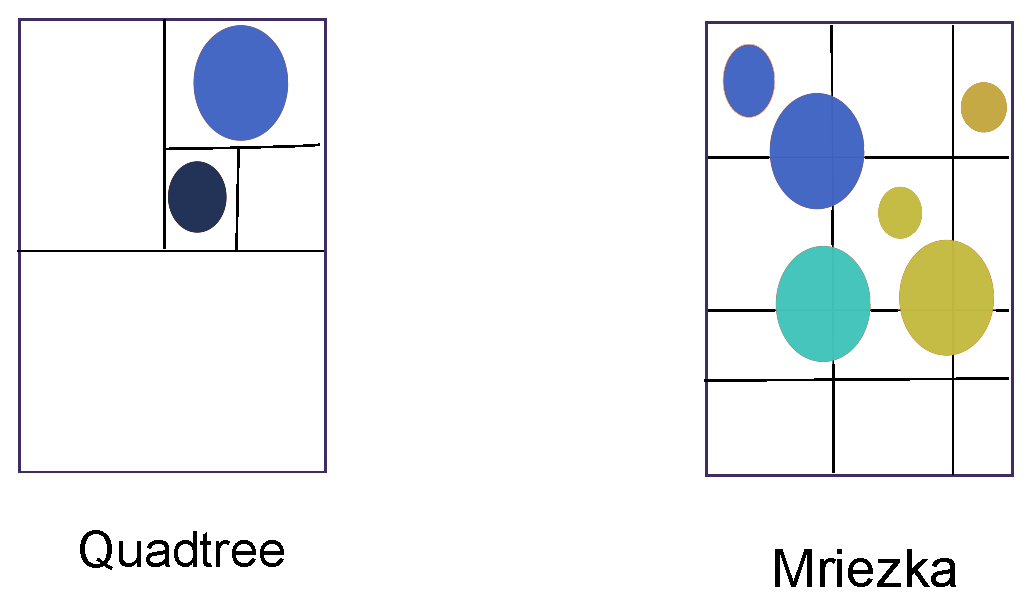
\includegraphics[totalheight=0.2\textheight,width=.2\textwidth]{mriezka}
\caption { Mriežková metóda. Objekty s rovnakou farbou patria do rovnakej oblasti}
\label{fig:hash}
\end{figure}
\indent Dosť často je využívaným spôsobom pre riešenie kolízií v 2D (3D) hrách je štruktúra zvaná quadtree. Quadtree je strom rozdeľujúci priestor na niekoľko častí podobne ako v mriežkovom spôsobe, na základe dostatočnej 'blizkosti' objektu, rozdiel spočíva v prístupe k informáciam a dynamickým vytváraním ďalších buniek. Na začiatku tvorí celý priestor jednu veľkú buňku. V okamihu, keď sa do buňku dostane istý počet objektov považovaný za maximálny, buňka sa rozdelí. Podobne, pokiaľ objekt prejde z jednej buňku do druhej a v pôvodnej už nezostáva nič, buňka zanikne (zostane už iba naradená, väčšia buňka). Samotná kolízia sa vypočíta podobne ako v predchádzajúcej metóde. Pekný tutoriál k implementácií Quadtree sa dá  nájst v \cite{quadtree}. Výhodou tejto implementácie je rýchlosť spracovania pre objekty rôznych veľkostí, poťažne a sú objektky zhlukované do malých oblastí.
\begin {figure}
\centering
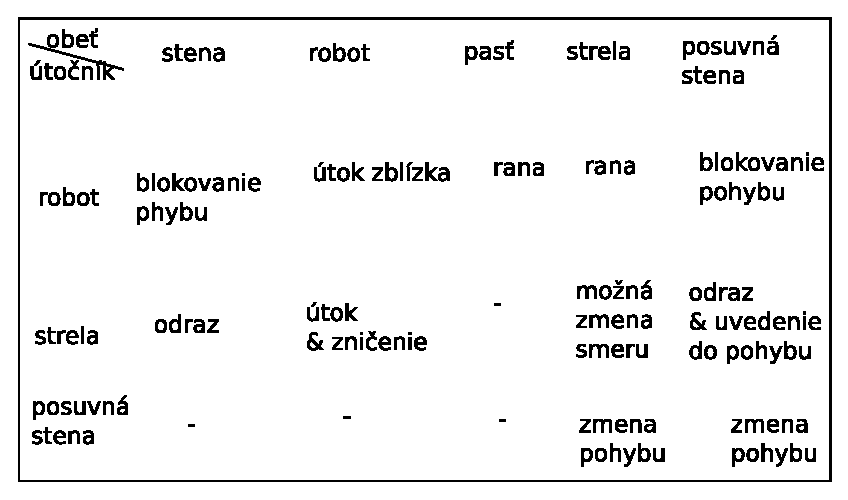
\includegraphics{kolizie}
{ Výsledok kolízii medzi rôznymi objektami }
\label{fig:kol}
\end {figure}

\subsection{ Definovanie skončenia misie }
Ako bolo spomenuté v požiadavkách, niektoré hry nepovažujú za důležité len prežitie robota v prostredí, ale musia byť splnené aj dodatočné podmienky. Preto v algoritme robota musí existovať ak sekvenia znakov, ktorá ich umožňuje dodatočne definovať. Vyvstáva otázka, prečo by tieto podmienky nemohli byť definované aj globálne, teda mimo algoritmu. Odpoveďou je, že s neuplnou informáciou sa dobré algoritmu píšu pomerne ťažko.\\% o to sakra melem???
Definovanie vítazného stavu sa v pro písaní programu pre robota objaví ešte pred funkciami v tvare:
\begin{itemize}
\item $Killed\ [>, < <=, >=, !=, ==]\ N, N \in Z$ , kde Killed je počet zabitých nepratieľov. Do tohoto počtu sa nezapočítavajú rozbité steny ani strely.
\item $Killed( N ), N \in [a-zA-Z0=9\_]*$ , kde N je identifikačný názov robota. Tento názov zadá užívateľ pre lepšiu identifikáciu algoritmu robota. Meno robota sa vyhľadá po naloadovaní všetkých vstupov. Ak sa toto meno nenájde, potom sa podmienka ignoruje.
\item $Visit([X,Y], [Z,W],..)$, kde X,Y sú súradnice miesta, ktoré musí robot prekročiť, v akomkoľvek poradí. Neprípustné hodnoty sa nekontrolujú, keďže v čase definovania misie nie je známa mapa, kde bude
\item $VisitSequence([X,Y], [Z,W],..)$, kde X,Y sú súradnice miesta, ktoré musí robot prekročiť, práve v tomto poradí. V prípade, že je definovaných viac takýchto inštrukcií, spracovávajú sa všetky simultánne, t.j ak má pravidlá definované ako v tabuľke \ref{tab:pr1} a pristúpi na políčko [20,20], splní sa v druhej sekvencii prvé miesto. Ak robot už predtým navštívil políčko [10,10], potom je kompletne splnená prvá podmienka a časť druhej. Opäť sa nekontrolujú neprípustné hodnoty vzhľadom na absenciu informácií o mape.
\item $Visit(X, Y,...); X,Y \in N $, kde X,Y sú čísla miest, ktoré musí robot navšíviť, v akomkoľvek poradí. Tieto čísla budú teda definované v mape
\item $VisitSequence(X,Y...0 X,Y \in N$, kde X,Y sú tiež čísla miest, ktoré musí robot navštítiť, ale v presne danom poradí.
\end{itemize}
V tabuľke \ref{tab:allVis} je prehľad všetkých zápisov cieľov, aké sú možné. Tieto ciele je možné pre vyššiu variabilitu kombinovať. Dopredná kontrola splniteľnosti cieľov nie je žiadúca, pretože až na triviálne prípady sa výsledok dá zistiť až po prebehnutí simulácie, čo je vlastne spor.
\begin{table}
\centering
\begin{tabular}{l}
VisitSequence([10,10],[20,20])\\
VisitSequence([20,20],[20,30])\\
\end{tabular}
\caption {Príklad 1 : pravidlá definujúce cieľ robota} %TODO figure!
\label{tab:pr1}
\end{table}

\begin{table}
\centering
\begin{tabular}{l}
VisitSequence([10,10],[20,20])\\
Visit([20,20],[20,30],[20,30])\\
$Kill < 4$\\
$Kill >= 5$\\
$Kill \!= 3$\\
$Kill == 8$\\
$Kill > 8$\\
$Kill <= 8$\\
$Visit([20,20],2,0)$\\
\end{tabular}
\caption {Príklad 2 : príklady pre pravidlá na definovanie cieľa} %TODO figure!
\label{tab:allVis}
\end{table}

V týchto podmienkach je ešte možné použiť premennú 'Start', ku ktorej sa pristupuje ako k poľu a označuje štartovnú pozíciu i-teho robota.\\
Kód, ktorý by simuloval populárnu hru 'Capture the flag' by napríklad vyzeral takto pre robota s menom Bot a súpera s menom AnotherBot:\\
\begin{table}
\centering
\begin{tabular}{l c}
VisitSequence(start[AnotherBot],start[Bot]) &\\ 
main()\\
\{\\
& turn(direction(getTarget()));\\
& move(100)\\
\}\\
\end{tabular}
\caption{ Príklad na simuláciu hry Capture the flag }
\end{table}

\subsection {Priebeh simulácie}
Hra sa začína umiestnením robotov do prostredia v poradí, v akom boli pridaní. Kvôli rovnosti šancí by mali roboti začať vykonávať svoj program súčasne. To však technicky nie je možné, takže je nutné zamaskovať to tým spôsobom, že sa vyhodnotia všetky akcie a v ďalšej fázi sa vyhodnotia naraz všetky výsledky. \\
 Priebeh simulácie codewars teda prebieha v nasledujúcich krokoch:
\begin {enumerate}
\item Vyberú a spracujú sa vstupy robotov.
\item Vstupy skontrolujú na syntaktické chyby, doplnia a skontrulú sa nastavenia vlastností robotov.
\item Roboti sa umiestnia na štartovacie políčka. Ak nie je dostatok štartovacích políčok, pokúsia sa umiestniť náhodne. Ak sa nepodarí ani to, dotyčný robot vypadáva zo simulácie. Pozícia štartu robota nesmie kolidovať s iným objektom. Ak koliduje, nie je považovaná za validné štartovacie políčko a robot sa tam neumiestni.
\item Priebieha kolo – každý robot oznámi, akú časť kódu chce vykonávať. 
\item Vypočítajú a vykreslia sa výsledky robotích akcií a objektov na mape ( pohyb objektov, zasiahnutie, vypočítanie škody, odstránenie častí so životnosťou menšou ako 0 ).
\item Skontroluje sa splnenosť cieľov u každého robota. Ak má aspoň jeden robot splnené všetky ciele, alebo ako jediný z robotov má životnosť väčšiu ako 0, simulácia skočí výpisom robotov, ktorí úspešne ukončili simuláciu. Inak sa pokračuje krokom 4.
\end{enumerate}

